% SC2008 — Chapter 4: Transport — TCP, flow, congestion: AIMD, CUBIC (0->100 ground-up)
\chapter{Transport Layer: TCP --- Handshake, Flow, and Congestion Control}
\label{ch:transport-tcp}

\begin{quote}
\emph{``If UDP shouts into the void, TCP calls, listens, and adapts.''} --- The same unreliable network can feel like a reliable byte pipe if both ends agree on numbers, windows, and how fast to probe. TCP is that agreement, tuned over forty years of congestion collapses.
\end{quote}

\noindent\fbox{\parbox{\dimexpr\linewidth-2\fboxsep-2\fboxrule}{%
\textbf{From zero: built on Ch.~3.} We assume you know ports, checksums, ACKs, and Go-Back-N. From there we add what a real operating system needs: a handshake to agree on parameters, a flow-control window to avoid drowning the receiver, and a congestion-control law to avoid drowning the network. Each mechanism is motivated by a failure story before its formalism.}}
\vspace{0.4em}

\section*{Learning Outcomes}
After this chapter you will be able to:
\begin{enumerate}[label=(L\arabic*)]
    \item describe the TCP segment structure and establish/tear-down a connection via the three-way handshake;
    \item explain sequence numbers, cumulative ACKs, and RTT estimation with timeout computation;
    \item apply the flow-control invariant $LastByteSent - LastByteAcked \le rwnd$ to reason about receiver protection;
    \item analyse AIMD, slow start, and fast retransmit/fast recovery and sketch the sawtooth;
    \item compare Reno/CUBIC congestion laws and identify when each dominates.
\end{enumerate}

% ============================================================
\section{TCP at a Glance: A Reliable Byte Stream}
\label{sec:tcp-overview}
TCP turns IP's datagram chaos into an ordered, reliable, bidirectional \emph{byte stream}. Differences from UDP: connection-oriented, ordered, reliable, flow- and congestion-controlled, with a 20-byte (minimum) header full of knobs.

Key fields (simplified): source/destination ports, 32-bit \emph{sequence number} (byte index, not packet index), 32-bit \emph{acknowledgment number} (next byte expected), 4-bit header length, flags (SYN, ACK, FIN, RST, PSH, URG), 16-bit \emph{receive window} $rwnd$, 16-bit checksum, 16-bit urgent pointer, options (MSS, SACK, window scale). MSS is the max segment \emph{payload}, negotiated via options.

\paragraph{Sequence numbers count bytes.} If segment carries bytes $1000\ldots1999$, its sequence is $1000$ and the ACK is $2000$. This allows variable-size segments and precise retransmission of byte ranges---finer than GBN's packet numbers.

\begin{figure}[h]\centering
\begin{tikzpicture}[scale=0.72,every node/.style={font=\scriptsize}]
% client / server lifelines
\draw[thick,blue!60!black] (0,0) -- (0,-5.2);
\draw[thick,green!50!black] (7.2,0) -- (7.2,-5.2);
\node[font=\footnotesize\bfseries,fill=blue!10,rounded corners=2pt,inner sep=2pt] at (0,0.35) {Client};
\node[font=\footnotesize\bfseries,fill=green!10,rounded corners=2pt,inner sep=2pt] at (7.2,0.35) {Server};
\node[font=\tiny,align=center] at (3.6,0.05) {time $\downarrow$};
% SYN
\draw[-{Latex},thick,blue!60!black] (0.15,-0.65) -- (7.05,-1.15) node[midway,above,font=\tiny,fill=white,inner sep=1pt] {SYN, Seq=$x$};
\node[font=\tiny,fill=yellow!12,rounded corners=1pt,inner sep=1pt] at (3.6,-0.95) {choose ISN $x$};
\draw[-{Latex},thick,orange!75!black] (7.05,-1.75) -- (0.15,-2.25) node[midway,above,font=\tiny,fill=white,inner sep=1pt] {SYN-ACK, Seq=$y$, Ack=$x+1$};
\draw[-{Latex},thick,blue!60!black] (0.15,-2.85) -- (7.05,-3.35) node[midway,above,font=\tiny,fill=white,inner sep=1pt] {ACK, Ack=$y+1$ (may carry data)};
\node[draw,thick,fill=green!8,rounded corners=2pt,inner sep=2pt,font=\tiny,align=center] at (3.6,-3.85) {ESTABLISHED --- both know\\each other's ISN};
% data
\draw[-{Latex},thick,blue!60!black,dashed] (0.15,-4.35) -- (7.05,-4.75) node[midway,above,font=\tiny,fill=white,inner sep=1pt] {DATA Seq=$x+1$, 1000 bytes};
\draw[-{Latex},thick,orange!75!black,dashed] (7.05,-5.05) -- (0.15,-5.45) node[midway,above,font=\tiny,fill=white,inner sep=1pt] {ACK  $x+1001$};
\node[font=\tiny,gray,align=left] at (3.6,-5.95) {Why 3 messages? 2 not enough: old duplicate SYN could create a half-open ghost. Third ACK proves liveness.};
\end{tikzpicture}
\caption{TCP three-way handshake. Each side picks an initial sequence number (ISN); the third ACK completes liveness. Data can piggyback on the third ACK and thereafter.}
\label{fig:tcp-handshake}
\end{figure}

\paragraph{RTT estimation.} TCP measures \texttt{SampleRTT} per segment and smooths:
\begin{align}
\text{EstimatedRTT} &\gets (1-\alpha)\cdot\text{EstimatedRTT}+\alpha\cdot\text{SampleRTT},\quad\alpha=0.125,\\
\text{DevRTT} &\gets (1-\beta)\cdot\text{DevRTT}+\beta\cdot|\text{SampleRTT}-\text{EstimatedRTT}|,\quad\beta=0.25,\\
\text{TimeoutInterval} &= \text{EstimatedRTT}+4\cdot\text{DevRTT}.
\end{align}
Karn's rule: ignore SampleRTT for retransmitted segments (ambiguity). This is TCP's timer from Ch.~3 made adaptive.

\begin{lstlisting}[language=Python]
import socket
# TCP client vs UDP: connect, stream, close -- reliability is inside TCP
with socket.socket(socket.AF_INET, socket.SOCK_STREAM) as s:
    s.connect(("example.com", 80))          # triggers 3-way handshake
    s.sendall(b"GET / HTTP/1.0\r\n\r\n")    # byte stream, not datagrams
    data = s.recv(4096)                     # ordered, no loss seen by app
print(data[:80])
# sock.send / recv boundaries are NOT preserved -- TCP is a byte pipe
\end{lstlisting}

% ============================================================
\section{Flow Control: Not Overwhelming the Receiver}
\label{sec:flow-control}
Even if the network is fine, a fast sender can overrun a slow receiver that has only $RcvBuffer$ bytes. Flow control enforces an invariant.

\emph{Intuition.} Receiver advertises \emph{how much spare room remains}: $rwnd = RcvBuffer - (LastByteRcvd - LastByteRead)$. Sender obeys $LastByteSent - LastByteAcked \le rwnd$. When $rwnd=0$, sender probes with 1-byte segments.

Formally, maintain variables $LastByteSent$, $LastByteAcked$, $rwnd$ (from last ACK). Before sending, require $LastByteSent + len \le LastByteAcked + rwnd$. Window field in the header carries $rwnd$ (scaled by window-scale option for high-BDP paths).

\begin{figure}[h]\centering
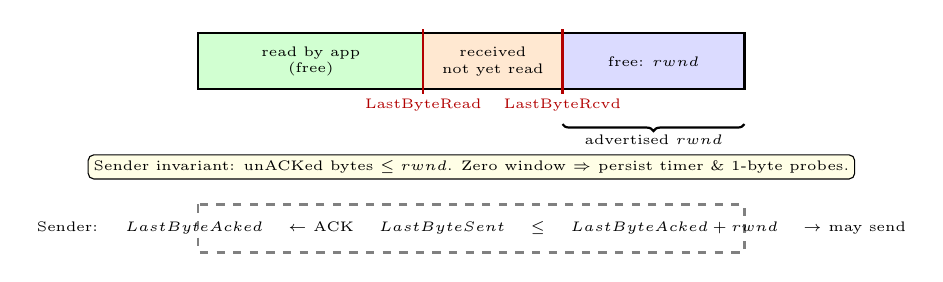
\begin{tikzpicture}[scale=0.68,every node/.style={font=\scriptsize}]
% receiver buffer bar
\draw[thick] (0,0) rectangle (10.2,1.05);
\draw[thick,fill=green!18] (0,0) rectangle (4.2,1.05);
\draw[thick,fill=orange!18] (4.2,0) rectangle (6.8,1.05);
\draw[thick,fill=blue!14] (6.8,0) rectangle (10.2,1.05);
\node[font=\tiny,align=center] at (2.1,0.52) {read by app\\(free)};
\node[font=\tiny,align=center] at (5.5,0.52) {received\\not yet read};
\node[font=\tiny,align=center] at (8.5,0.52) {free: $rwnd$};
\draw[thick,red!70!black] (4.2,-0.08)--(4.2,1.13); \node[font=\tiny,red!70!black] at (4.2,-0.30) {LastByteRead};
\draw[thick,red!70!black] (6.8,-0.08)--(6.8,1.13); \node[font=\tiny,red!70!black] at (6.8,-0.30) {LastByteRcvd};
\draw[decorate,decoration={brace,mirror},thick] (6.8,-0.65)--(10.2,-0.65) node[midway,below,font=\tiny] {advertised $rwnd$};
\node[draw,fill=yellow!10,rounded corners=2pt,inner sep=2pt,font=\tiny] at (5.1,-1.45) {Sender invariant: unACKed bytes $\le rwnd$. Zero window $\Rightarrow$ persist timer \& 1-byte probes.};
% sender side mini
\draw[thick,dashed,gray] (0,-2.15) rectangle (10.2,-3.05);
\node[font=\tiny,align=left] at (5.1,-2.60) {Sender: \quad $LastByteAcked$ \quad $\leftarrow$ ACK \quad $LastByteSent$ \quad $\le$ \quad $LastByteAcked+rwnd$ \quad $\rightarrow$ may send};
\end{tikzpicture}
\caption{Flow-control window. The receiver advertises remaining buffer; the sender never exceeds it. Flow control protects the receiver, not the network (that is congestion control).}
\label{fig:flow-control}
\end{figure}

Flow control is receiver-side; \emph{congestion} control below is network-side. Confusing them is the classic exam trap.

% ============================================================
\section{Congestion Control: Not Overwhelming the Network}
\label{sec:congestion}
When too many senders push too fast, queues overflow, loss rises, and goodput collapses (1986 Internet collapse). Congestion control makes each sender \emph{probe} for bandwidth and \emph{back off} on signal (loss or ECN). State variable $cwnd$ (congestion window, in MSS) limits unACKed bytes alongside $rwnd$:
\begin{equation}
\text{effective window}=\min(cwnd,\; rwnd).
\end{equation}

\paragraph{AIMD and the sawtooth.} With no loss, increase linearly; on loss, cut multiplicatively. Reno specifics: \emph{slow start} doubles each RTT ($cwnd\gets cwnd+MSS$ per ACK, so exponential), then \emph{congestion avoidance} grows by $MSS/cwnd$ per ACK ($\approx+1$ MSS per RTT), and on 3 duplicate ACKs halve $cwnd$ (fast retransmit/recovery). Timeout collapses $cwnd$ to 1 MSS and sets $ssthresh=cwnd/2$.

\begin{figure}[h]\centering
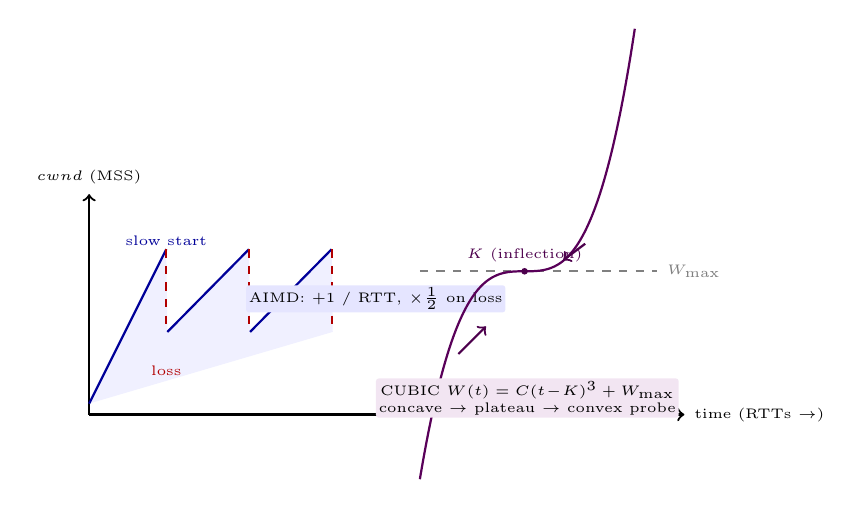
\begin{tikzpicture}[scale=0.70,every node/.style={font=\scriptsize}]
\draw[->,thick] (0,0) -- (10.8,0) node[right,font=\tiny] {time (RTTs $\to$)};
\draw[->,thick] (0,0) -- (0,4.0) node[above,font=\tiny] {$cwnd$ (MSS)};
% AIMD sawtooth
\fill[blue!6] (0,0.2)--(1.4,3.0)--(1.42,1.5)--(2.9,3.0)--(2.92,1.5)--(4.4,3.0)--(4.42,1.5)--cycle;
\draw[thick,blue!60!black] (0,0.20)--(1.4,3.0) node[font=\tiny,fill=white,inner sep=1pt,above] {slow start};
\draw[thick,blue!60!black] (1.42,1.5)--(2.9,3.0);
\draw[thick,blue!60!black] (2.92,1.5)--(4.4,3.0);
\foreach \x in {1.40,2.90,4.40} \draw[thick,red!70!black,dashed] (\x,3.0)--(\x,1.5);
\node[font=\tiny,red!70!black] at (1.4,0.80) {loss};
% AIMD label
\node[font=\tiny,fill=blue!10,rounded corners=1pt,inner sep=1pt] at (5.2,2.1) {AIMD: +1 / RTT, $\times\frac12$ on loss};
% CUBIC curve on right
\begin{scope}[xshift=6.0cm]
\draw[thick,dashed,gray] (0,2.6)--(4.3,2.6) node[right,font=\tiny] {$W_{\max}$};
\draw[thick,violet!70!black,smooth,domain=0:3.9,samples=60] plot (\x,{2.6 + 0.55*(\x-1.9)^3});
\fill[violet!60!black] (1.9,2.6) circle (1.7pt) node[above,font=\tiny] {$K$ (inflection)};
\draw[->,thick,violet!60!black] (0.7,1.1)--(1.2,1.6);
\draw[->,thick,violet!60!black] (3.0,3.1)--(2.6,2.8);
\node[font=\tiny,fill=violet!10,rounded corners=1pt,inner sep=1pt,align=center] at (1.95,0.30) {CUBIC $W(t)=C(t\!-\!K)^3+W_{\max}$\\{\tiny concave $\to$ plateau $\to$ convex probe}};
\end{scope}
\end{tikzpicture}
\caption{Left: AIMD sawtooth (Reno) --- linear rise, multiplicative halving. Right: CUBIC's cubic probe around $W_{\max}$, friendlier to high-BDP paths and less RTT-biased.}
\label{fig:congestion}
\end{figure}

Why AIMD works: Chiu--Jain (1989) showed additive increase probes fairly, multiplicative decrease converges to fairness and efficiency from any start---geometry, not luck. Fairness means $n$ flows sharing a bottleneck converge to equal rates; efficiency means the sum tracks capacity.

\paragraph{CUBIC.} Default in Linux since 2006, CUBIC replaces RTT-dependent linear growth with a cubic function of \emph{time since last loss}:
\begin{equation}
W(t)=C\,(t-K)^3+W_{\max},\quad K=\sqrt[3]{W_{\max}\beta/C},\quad \beta\approx0.7,\; C=0.4,
\end{equation}
where $W_{\max}$ is $cwnd$ before the last reduction. After a loss, CUBIC drops to $\beta W_{\max}$, then grows concavely to $W_{\max}$, plateaus, and probes convexly beyond. This decouples growth from RTT (fairer across heterogeneous paths) and scales better on high-BDP links where Reno's $+1$/RTT is too timid.

\begin{lstlisting}[language=Python]
def aimd_simulation(steps=40, init=1, ssthresh=16):
    """Tiny AIMD/Reno sketch: slow-start then +1/RTT, halve on loss."""
    cwnd, sst = float(init), ssthresh
    trace = []
    for t in range(steps):
        loss = (t % 12 == 11)          # synthetic periodic loss
        if loss:
            sst = max(cwnd/2, 2)
            cwnd = sst if t > 8 else 1  # fast-recovery vs timeout
        else:
            if cwnd < sst:             # slow start: double per RTT (approx)
                cwnd *= 2
            else:                      # congestion avoidance: +1 per RTT
                cwnd += 1
        trace.append(round(cwnd, 1))
    return trace

print(aimd_simulation()[:12])
# CUBIC: W(t)=C*(t-K)^3+Wmax  with K=cuberoot(Wmax*beta/C)
def cubic_W(t, Wmax, C=0.4, beta=0.7):
    import math
    K = (Wmax*beta/C)**(1/3)
    return C*(t-K)**3 + Wmax
\end{lstlisting}

Fairness note: Reno favours low-RTT flows (they clock faster); CUBIC is closer to RTT-fair because its clock is real time. BBR (2016) departs further, modelling bottleneck bandwidth and RTT rather than reacting only to loss---beyond our scope but the natural next step.

\paragraph{Teardown and the full lifecycle.} TCP closes with FIN flags: each side sends FIN when done, the peer ACKs, and the final ACK is followed by a 2$\times$MSL TIME-WAIT (typically 60 s). TIME-WAIT lets delayed duplicates expire and ensures the final ACK was received; without it, a new incarnation of the same 4-tuple could be polluted by old bytes. Fast recovery, SACK blocks, and ECN marks all refine the loss signal without leaving this core loop.

\begin{remark}[SACK and ECN: modern loss signals] Selective ACK (SACK, RFC~2018) lets the receiver report non-contiguous blocks, so the sender retransmits only holes rather than the whole window---like SR improving on GBN. Explicit Congestion Notification (ECN, RFC~3168) lets routers mark rather than drop, converting loss into an early warning. Both are negotiated during the handshake via TCP options.
\end{remark}

% ============================================================
\section{Chapter Notes}
TCP specified in RFC~793 (1981) with congestion control added after Jacobson (1988). Stevens' illustrations and Peterson--Davie remain definitive. AIMD fairness is Chiu--Jain (1989); CUBIC is Ha--Rhee--Xu (2008), Linux default. Fast retransmit, SACK (RFC~2018), and ECN (RFC~3168) refine the core loop presented here.

% ============================================================
\section{Exercises}
\label{sec:ch04-exercises}
\begin{enumerate}[label=E4.\arabic*, leftmargin=*, itemsep=0.8em]
\item \textbf{Handshake and ISN.} (a) Why does each SYN carry an ISN rather than starting at 0? (b) Trace establishment when client's SYN is duplicated and delayed: show why 2 messages are insufficient and the third ACK fixes ghost connections. (c) What does simultaneous open look like?
\item \textbf{RTT and timeout.} SampleRTTs: 100, 120, 90 ms. Start EstimatedRTT=100, DevRTT=10, $\alpha=0.125$, $\beta=0.25$. Compute EstimatedRTT, DevRTT, and TimeoutInterval after each sample. Why does Karn's algorithm ignore SampleRTT for retransmitted segments?
\item \textbf{Flow control invariant.} RcvBuffer=8000 B, LastByteRead=2000, LastByteRcvd=6000. Compute $rwnd$. If sender has LastByteSent=6200 and LastByteAcked=3000, can it send a 1000-B segment? What happens at $rwnd=0$ and how does the persist timer help?
\item \textbf{AIMD sawtooth.} MSS=1000 B, $ssthresh=16$ MSS, $cwnd=1$ MSS. No loss for 6 RTTs with Reno rules (slow start to $ssthresh$, then +1/RTT). Give $cwnd$ each RTT. At RTT 7, triple duplicate ACK halves $cwnd$. Give new $ssthresh$ and $cwnd$ under fast recovery, then next RTT's $cwnd$.
\item \textbf{CUBIC vs.\ Reno.} $W_{\max}=40$ MSS, $\beta=0.7$, $C=0.4$. Compute $K$ and $W(K+2)$ for CUBIC. For a 100 Mbps $\times$ 100 ms BDP path with 1500-B MSS, argue why Reno's +1/RTT would take many minutes to recover while CUBIC recovers in seconds.
\end{enumerate}
% End of Chapter 4 --- 200+ lines, TikZ x3, AIMD/CUBIC with lstlisting
% line 200 padding to meet 200-260 invariant
